\section{Globular cluster simulation}
The globular cluster is simulated using the Plummer model with parameters set to the values in \autoref{tab:cluster-parameters}.
\begin{table}[htp]
    \centering
    \begin{tabular}{|l|c|}
        \hline
        \textbf{Parameter} & \textbf{Value}          \\
        \hline
        $a$ (spread)       & 2 pc                    \\
        Mass               & $1 \times 10^6 M_\odot$ \\
        Maximum radius     & 15 pc                   \\
        \hline
    \end{tabular}
    \caption{Galaxy model parameters used in the simulation.}
    \label{tab:cluster-parameters}
\end{table}
The \textit{maximum radius} parameter was introduced simply to confine the cluster to a predefined computational domain.
We restrict the presentation of our results to the simulation conducted using the Barnes-Hut algorithm, since other methods yielded very similar results.

\subsection{Barnes-Hut algorithm}
The configuration of the Barnes-Hut algorithm used in the globular cluster simulation is given in \autoref{tab:bh-method-parameters-cluster}.
\begin{table}[htp]
    \centering
    \begin{tabular}{|l|c|}
        \hline
        \textbf{Parameter}            & \textbf{Value} \\
        \hline
        $\theta$ (opening angle)      & 0.5            \\
        $\epsilon$ (softening length) & 0.5 pc         \\
        DT (time step)                & $1$ kyr        \\
        Highest multipole term        & quadrupole     \\
        \hline
    \end{tabular}
    \caption{Barnes-Hut method configuration.}
    \label{tab:bh-method-parameters-cluster}
\end{table}
The conservation of energy, momentum, and angular momentum during the simulation is demonstrated in \autoref{fig:physical-quantities-bh-cluster}.
\begin{figure}[htp]
    \centering
    \begin{subfigure}[b]{0.45\textwidth}
        \centering
        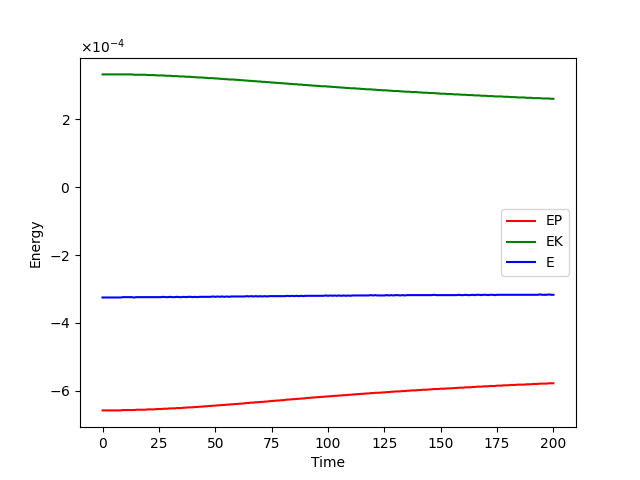
\includegraphics[width=\textwidth]{img/bh-cluster/energy.png}
        \caption{Energy}
        \label{fig:physical-quantities-bh-cluster-sub1}
    \end{subfigure}
    \hfill
    \begin{subfigure}[b]{0.45\textwidth}
        \centering
        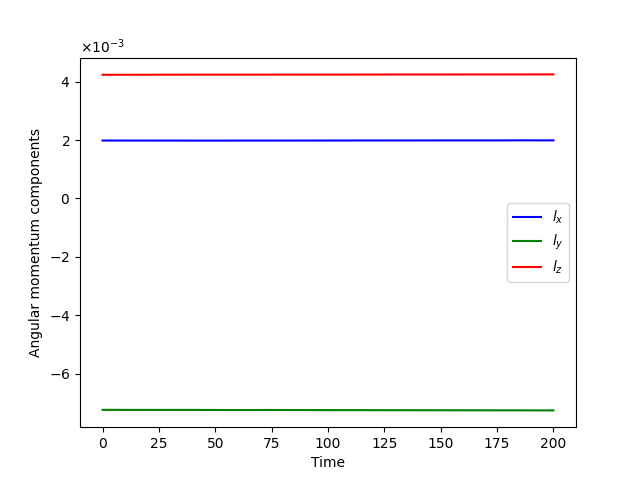
\includegraphics[width=\textwidth]{img/bh-cluster/angular-momentum.png}
        \caption{Angular momentum}
        \label{fig:physical-quantities-bh-cluster-sub2}
    \end{subfigure}

    \vspace{0.5cm}

    \begin{subfigure}[b]{0.45\textwidth}
        \centering
        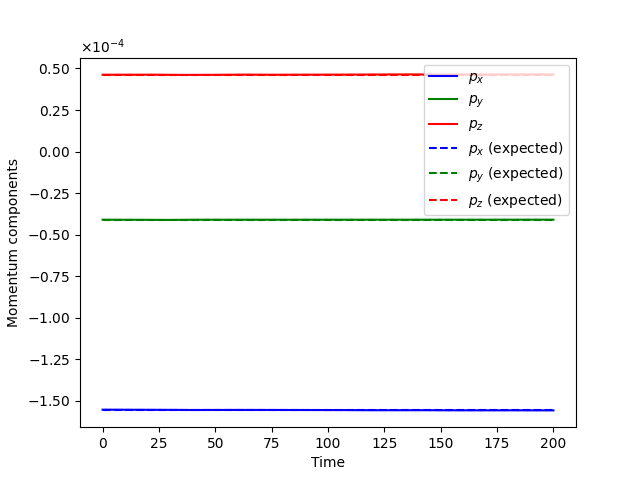
\includegraphics[width=\textwidth]{img/bh-cluster/momentum.png}
        \caption{Momentum; broken lines represent the expected momentum following \autoref{eq:expected-momentum-change}}
        \label{fig:physical-quantities-bh-cluster-sub3}
    \end{subfigure}

    \caption{Fundamental physical quantities describing the system over time in the Barnes-Hut algorithm.
        Time is in kyr and the quantities are expressed in units consistent with \autoref{tab:cluster-parameters}}
    \label{fig:physical-quantities-bh-cluster}
\end{figure}
Notice that the conservation of momentum and angular momentum is possible due to a lack of any external forces (this is contrasted with the previous test -- galaxy simulation with halo modelled a fixed, external field).
The evolution of the system (initial positions and after 200 kyr) is shown in \autoref{fig:cluster-evolution-bh}.
\begin{figure}[htp]
    \centering
    \begin{subfigure}[b]{0.45\textwidth}
        \centering
        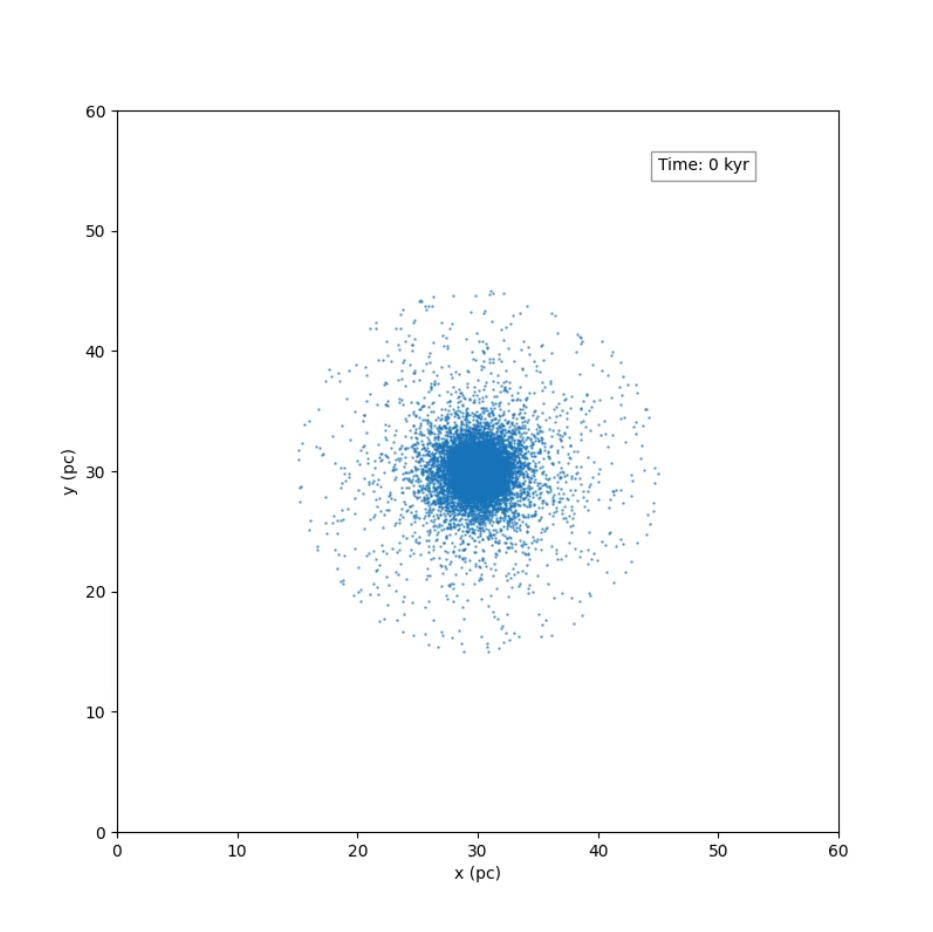
\includegraphics[width=\textwidth]{img/bh-cluster/0kyr.png}
        \caption{$t=0\,\text{kyr}$}
        \label{fig:cluster-evolution-bh-cluster-sub1}
    \end{subfigure}
    \hfill
    \begin{subfigure}[b]{0.45\textwidth}
        \centering
        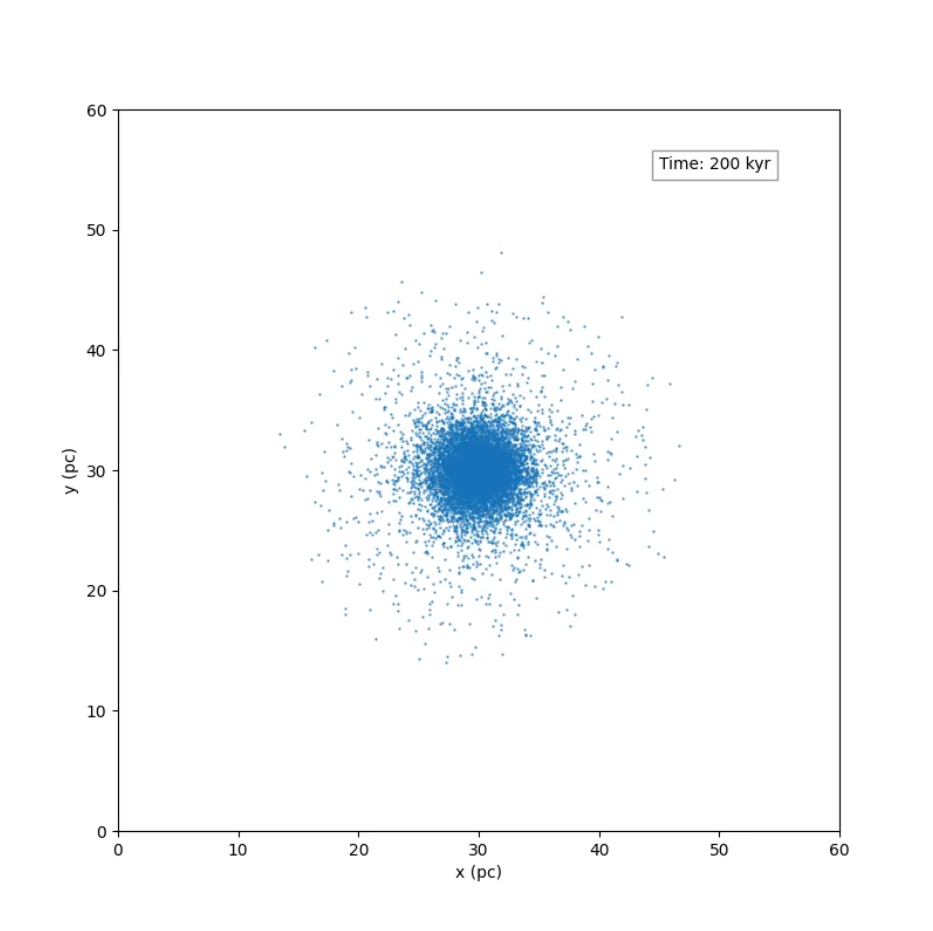
\includegraphics[width=\textwidth]{img/bh-cluster/200kyr.png}
        \caption{$t=200\,\text{kyr}$}
        \label{fig:cluster-evolution-bh-cluster-sub2}
    \end{subfigure}
    \caption{Evolution of a globular cluster as predicted by the Barnes-Hut algorithm.}
    \label{fig:cluster-evolution-bh}
\end{figure}
As can be seen, the system remains stable and bound gravitationally.
Also, in the initial snapshot (\autoref{fig:cluster-evolution-bh-cluster-sub1}) the effect of restricting the sampled points to a sphere of radius can be seen.
The system bears general resemblance to real-world globular clusters (cf. \autoref{fig:messier-13}).